\documentclass[10pt,letterpaper]{article}
\usepackage[top=0.85in,left=2.75in,footskip=0.75in]{geometry}

\usepackage[version=4]{mhchem}

% amsmath and amssymb packages, useful for mathematical formulas and symbols
\usepackage{amsmath,amssymb}

% Use adjustwidth environment to exceed column width (see example table in text)
\usepackage{changepage}

% Use Unicode characters when possible
\usepackage[utf8x]{inputenc}

% textcomp package and marvosym package for additional characters
\usepackage{textcomp,marvosym}

% cite package, to clean up citations in the main text. Do not remove.
\usepackage{cite}

% Use nameref to cite supporting information files (see Supporting Information section for more info)
\usepackage{nameref,hyperref}

% line numbers
\usepackage[right]{lineno}

% ligatures disabled
\usepackage{microtype}
\DisableLigatures[f]{encoding = *, family = * }

% color can be used to apply background shading to table cells only
\usepackage[table]{xcolor}

% array package and thick rules for tables
\usepackage{array}

% create "+" rule type for thick vertical lines
\newcolumntype{+}{!{\vrule width 2pt}}

% create \thickcline for thick horizontal lines of variable length
\newlength\savedwidth
\newcommand\thickcline[1]{%
  \noalign{\global\savedwidth\arrayrulewidth\global\arrayrulewidth 2pt}%
  \cline{#1}%
  \noalign{\vskip\arrayrulewidth}%
  \noalign{\global\arrayrulewidth\savedwidth}%
}

% \thickhline command for thick horizontal lines that span the table
\newcommand\thickhline{\noalign{\global\savedwidth\arrayrulewidth\global\arrayrulewidth 2pt}%
\hline
\noalign{\global\arrayrulewidth\savedwidth}}


% Remove comment for double spacing
%\usepackage{setspace} 
%\doublespacing

% Text layout
\raggedright
\setlength{\parindent}{0.5cm}
\textwidth 5.25in 
\textheight 8.75in

% Bold the 'Figure #' in the caption and separate it from the title/caption with a period
% Captions will be left justified
\usepackage[aboveskip=1pt,labelfont=bf,labelsep=period,justification=raggedright,singlelinecheck=off]{caption}
\renewcommand{\figurename}{Fig}

% Use the PLoS provided BiBTeX style
\bibliographystyle{plos2015}

% Remove brackets from numbering in List of References
\makeatletter
\renewcommand{\@biblabel}[1]{\quad#1.}
\makeatother



% Header and Footer with logo
\usepackage{lastpage,fancyhdr,graphicx}
\usepackage{epstopdf}
%\pagestyle{myheadings}
\pagestyle{fancy}
\fancyhf{}
%\setlength{\headheight}{27.023pt}
%\lhead{\includegraphics[width=2.0in]{PLOS-submission.eps}}
\rfoot{\thepage/\pageref{LastPage}}
\renewcommand{\headrulewidth}{0pt}
\renewcommand{\footrule}{\hrule height 2pt \vspace{2mm}}
\fancyheadoffset[L]{2.25in}
\fancyfootoffset[L]{2.25in}
\lfoot{\today}

%% Include all macros below

\newcommand{\lorem}{{\bf LOREM}}
\newcommand{\ipsum}{{\bf IPSUM}}

%% END MACROS SECTION


\begin{document}
\vspace*{0.2in}

% Title must be 250 characters or less.
\begin{flushleft}
{\Large
\textbf\newline{ A mechano-chemical compartment-based method to simulate the ameoboid movement} % Please use "sentence case" for title and headings (capitalize only the first word in a title (or heading), the first word in a subtitle (or subheading), and any proper nouns).
}
\newline
% Insert author names, affiliations and corresponding author email (do not include titles, positions, or degrees).
\\

a\textsuperscript{2\Yinyang},
b\textsuperscript{2\Yinyang},
c\textsuperscript{3},
d\textsuperscript{4},
e\textsuperscript{5},
Mehdi Sadeghi\textsuperscript{1*}

\bigskip
\textbf{1} National Institute of Genetic Engineering and Biotechnology (NIGEB), Tehran, Iran
\\
\textbf{2} 

\textbf{3} 
\\
\textbf{4} 
\\
\textbf{5} 

\bigskip


% Insert additional author notes using the symbols described below. Insert symbol callouts after author names as necessary.
% 
% Remove or comment out the author notes below if they aren't used.
%
% Primary Equal Contribution Note
\Yinyang These authors contributed equally to this work. 

* sadeghi@nigeb.ac.ir



% Additional Equal Contribution Note
% Also use this double-dagger symbol for special authorship notes, such as senior authorship.
%\ddag These authors also contributed equally to this work.

% Current address notes
%\textcurrency Current Address: Dept/Program/Center, Institution Name, City, State, Country % change symbol to "\textcurrency a" if more than one current address note
% \textcurrency b Insert second current address 
% \textcurrency c Insert third current address

% Deceased author note
%\dag Deceased

% Group/Consortium Author Note
%\textpilcrow Membership list can be found in the Acknowledgments section.

% Use the asterisk to denote corresponding authorship and provide email address in note below.


\end{flushleft}
% Please keep the abstract below 300 words
\section*{Abstract}
\textbf{} \\~


\noindent \textbf{Keywords:} \textit{Dictiostelium discoiudium}, voxel-based simulation
\hspace{2in}



% Please keep the Author Summary between 150 and 200 words
% Use first person. PLOS ONE authors please skip this step. 
% Author Summary not valid for PLOS ONE submissions.   
%\section*{Author summary}
%The ability of cells to beget different types of cells, and the capacity of the cells to organize in an orderly fashion are innovations that led to the emergence of multicellular life forms. The molecular mechanisms used to explain the complexity of these phenomena makes it hard to understand them in an evolutionary context. Here we present a parsimonious model which attempts to explain differentiation and self-organization by taking into account the noisy environment that exists inside and outside a living cell.

\linenumbers

\section*{Introduction}
Motility is a survival evolutionary starategy  in eukaryotes\cite{Brunet-2016}. The ability requires the coordination of complex mechanisms on the microscopic level, including  transducing information from the external environment to the interior of the cell and translating it to a migratory response via a molecular signaling pathway based on enviromental cues. One can classifies motile cells to swimmers and crawlers. Crawling cells , unlike swimming ones, do not posses a segragated organel for their motility. Instead, they employ an internal mechanism to push their membrane and in consequence the whole body forward. Amoeboid locomotion is the most frequent mode of movement in eukaryotic cells. \textit{Dictyostelium discoideum} is a well-established  model organism  for studying amoeboid like motility. The cell extend sucsessive pseudopodia, a temporary actin-based protrusion of its surface in order to propel on the surface following the signaling messenger cyclic Adenosin Mono Phosphate (cAMP) gradient. \\
Chemotactic movement of \textit{Dictyostelium discoideum} can be divided into three different steps: (1) receptor binding (2) polarizing and directional sensing (3) and migration response~\cite{Devreotes-2003}. Experiments show that it takes less than 10 seconds for an individual to respond an external chemical field~\cite{Meili-2015}.
When the starved cell exposed to a gradient of the chemoattractant, extracellular cAMP stochasticly bindes to the  cAR1 receptors distributed homogeneously around the cell membrane. This, in turn, triggers internal pathway which leads to localization of different agents at the leading edge and rear side of the cell.  After the cell  sensed its direction, the pathway must be linked to the actin-machinery to generate forces in the cytoskeleton. Then, the cell starts to migrate towards that direction. %To produce the forces required for the motion, actin is often associated with myosin, as in muscles (Bray,2001). However, It is a widely held view that the the process of actin polymerization itself is sufficient to induce cell movement. Indeed, it has been shown that the existence of  myosin motor protein is not necessary to produce a motile force((Mitchison and Cramer, 1996).\\
 \\~
There are impressive studies trying to make theoretical grounds for different aspects of chemotaxis in \textit{Dictyostelium discoideum}. Local Excitation/Global Inhibition (LEGI) models extended to explain gradient sensing in migrating cells. The ability of living organism to produce adapted and amplified responses, traced back to a fast and local excitatory reply that accompanies with a slow and inhibitory signal\cite{leg1,leg2,leg3}. In more recent versions of LEGI based models, parallel mechanism are introduced to regulate the accumulation of $ PI3K $ and $ PTEN $ proteins in front and back of the cell\cite{leg4}. In polarization models, usually a diffusing inhibitor is present and positive feedback loops are used to amplify the response of the network \cite{pol6,pol7}. One main feature of polarization models is a distinct differentiation between anterior and posterior regions results from positive feedback loops. It is beleived that a complete picture of chemotaxis achieves when coupled directional sensing and polarization mechanisms are taken into account. It is shown that chemoattractant activation of divergent pathways that inhibit each other by interaction with actin polymers, is sufficient for both gradient sensing and polarization\cite{pol8}. Coupled exitable Ras and actin activation can mediate pseudopodia formations and directed movement\cite{cop1}. A common feature in chemotaxis models is a chemical pathway activated by G-proteins coupled to receptors. The identity of these pathways and the way in which they interact, is critical for undrestanding of directed movement of cells in inhomogeneous environments.\\  
 Polarized regions contains distinct molecules with different functions and sensitivity to gradient of chemoattractants. The true mechanisms of polarity are still under debate, however, positive feedback loops containing actin polymers may be responsible for generation of local polarized regions inside the cell\cite{pol1,pol2,pol3}. Observations shows that in polarized cells \textit{PI3K} molecules are localized in front and \textit{PTEN} molecules at the back of the cell\cite{pol4,pol5}. Joining polarization and directional sensing results to co-ordinated migration up to the attractant gradient.\\~ Cell migration is an ATP-consuming process  associated with actin polymerization. The complex process, couples  protrusion of the cell’s leading edge with contraction of the cytoskeleton during a dynamically graded adhesion with substrate. Adhesion with the substrate is a requisite property without which crawlers are unmoveable. Dictyostelium cells, unlike other mammalian cells, enjoy of some innate Non-Specific cell substratum adhesion originally mediated by van der Waals interactions~\cite{Rappel-2012}. \\~ The polarized cells exhibit correlated deformations in their contour with a complex moleclar mechanism interacting with substrate via adhision forces. The sequential interaction leads to a persistant movement, even in the homogeneous medium. Ofcourse, eventually, on long runs the statistic of their locomotion in such field showes a diffusive behavior.This spomtanaous directional sensing and persistant random walk in the absence of environmental chemical cues is due to internal and external noises. When exposed to chemically inhomogeneous medium, the cells display a tendency to align with the local gradient of stimulants. 


Previous works stands for modeling the trajectories of amoeboid cells by stochastic differential equations with parameters estimated from experimental data. Although the equations well-describe the cellular central mass dynamics, due to the large size of the cells ($  nearly\, 10 \mu m$) it comprises variant simplifications.  The directional sensing models also  presents more a generic (theoretical) scheme that could satisify the above mentioned properties of directional sensing . \\~

The living entities are not purpose-built artifacts, engeneered to consistantly perform an exact action in response to an incoming signal; rather a cell is more akin to a soup of ingreiedents coliding and aggreagting within cells. Local events in this animate soap should result in global actions, thus the key to decipher the behaviour of a living systems, is to understand how to collective effects of these local events can give rise to something that can be mistaken for the responce of an inanimate artifact with global roles.\\~
One of the major shortfalls of a globalist view of a cell, is the fact that a cell, especially of eukaryotic variety, is deeply compartmentalized, where the concentrations of different chemical species are drastically different from any two points in the cytocol. Here, to capture the compartmentalized nature of a living cell, we divide up our artificial cell into compartemnts of a fixed size, operting independently of each other.The size of these copmatemnts are such that a well-stirred environemnt for the chimical reactions occuring within them is availible. \\~



%Here we will develop this approach further to also capture the heterogeneity inside the cell by considering it as an extended body partitioned by ''voxels", a smaller well-stired unite in which the chemical reactions occure. This is a step forward to make the molecullar mechanism model more realistic. Moreover, it makes it possible to rebuild the mutation effects. \\


\section*{Materials and methods}

Modeling the movement of a single-celled organism is seemingly an insurmountable task; given the complexity if such behavior, a faithful recreation would be computational cul-da-sac. Instead we have chosen to study this behavior at two different levels: 

\begin{enumerate}

\item \textit{The chemical level}: at this level we simulate the chemical reaction in pre-defined compartments, ``voxels'', using the Gillespie's method. The formation of pseudopodia is net result of these reactions.

\item \textit{The mechanical level}: the collective outcome of the the chemical reactions is translated into Newtonian equations in order to transform the chemical level into the movement of a physical entity --i.e., the cell-- on a surface.
\end{enumerate}

The interaction between the chemical and the physical levels results in a fascinating charactristic that neither levels nor their building blocks can muster: the ability to respond to chemotactic cues present in its  enviorenment. This emergenet feature separates the realm of goal-less, unguided, and mindless objects from the realm of living entities that change their behaviors vis-${a}'$-vis their \textit{Umwelt}.

\subsection*{The chemical level}
Directed migration of primitive or elaborated living systems, can be followed from the analysis of physio-chemical properties of  chemotaxis process. From a hierarchical point of view, stimulation of cells with chemoattractants or intrinsic noise, triggers downstream chemical pathways induce polarization in motile cell. These complicated networks allows cells to detect external gradients. Difference in concentration of related agents, translates to physical forces at the outer level which are responsible for pushing the membrane forward and generating pseudopods. Any proposed model used to address chemotaxis problem throughly, should consider three steps: motility, directional sensing and polarity. Motility refers to propelling the cell in random directions probably due to external noise. Pseudopodia growth in arbitrary directions because of noisy behaviour of the environment. It seems the same chemical pathway works in the presence or absence of external stimuli. However, since noise exerts unidirectional forces, the movement of the cell is not biased in motile behaviour of cell. In directional sensing cells can differentiate between inhomogeneous distributions of chemoattractants. Directional sensing depends on the ability of cells to detect the change in the occupancy of receptors over time. It is known as temporal sensing provide cells to bias their movement by sensing the occupancy of receptors across the cell length. Sensing of gradients follows with the tendency of signals to reach a specific value during the saturation of receptors. It is said that responses \textit{adapts} to the external stimulus. Then, directional sensing consist in reading the extracellular gradient and transmitting information about spatio-temporal properties of attractants inside the cell. Where the content of this information translates to change in cell morphology and induce motility in a directed fashion. Polarization is crucial for moving to the gradient after receiving extracellular signals. In polarized cells spatial distribution of certain molecules are restricted to leading or lagging edge of the cell.\\

\begin{figure}
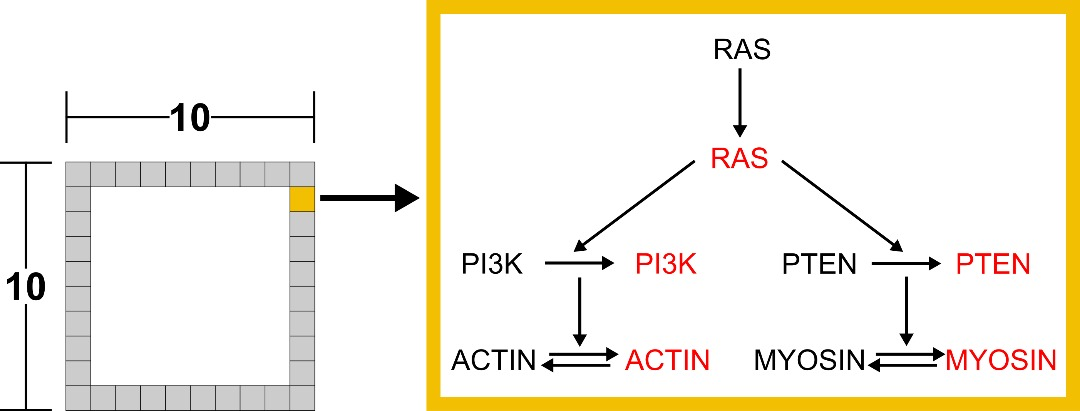
\includegraphics[scale=0.35]{Fig1.jpeg}
\caption{Chemical pathway for chemotaxis of \textit{Dictyostelium discoideum}.Propensity functions for stochastic solution of kinetic equations are given for related reactions.}
\label{Fig.1}
\end{figure}

In our proposed pathway, stimulation of receptors with binding of cAMP, or in the absence of external stimuli,  by fluctuations in the environment, activates transformation of $ Ras $ proteins into excited counterpart $ Ras^{\star}$. $ Ras^{\star} $ mediates transformation of deactivated $ PI3K $ and $ PTEN $ to their active forms $ PI3K^{\star} $ and $ PTEN^{\star} $.  Activation passes through intermediates species $ Ras^{\star}.PI3K $ and $ Ras^{\star}.PTEN $ decomposed to active forms and deposit $ PI3K $ and $ PTEN $ enzymes intact.
 $ PI3K^{\star} $ and $ PTEN^{\star} $ has the same role of $ Ras^{\star}$ for the polymerization reaction of actin monomers and contraction of at rest myosins, respectively. Polymerized actins $(Actin^{\star})$ and contracted myosins $ (Myosin^{\star}) $ can decompose to actin monomers and expanded myosins in backward reactions. $ PI3K^{\star}.Actin $ and $ PTEN^{\star}.Myosin $ faciliates the conversion of inactive actin-myosin molecules to their active forms.\\
We have used Gillespie algorithm for stochastic solution of chemical reactions. The main characteristics of the chemotaxis process, adaptation to signal, amplification in concentration of actin's activator and polarization of the cell due to difference in concentration of actin and myosin, are included in definitions of propensity functions of the reactions (see Fig.(\ref{Fig.1})). Following propensity functions, concentration of $ PI3K^{\star} $ amplifies \textit{linearly} with increase in concentration of cAMP and polymerized actin. Then, polymerization reaction can be considered as a positive feedback for activation of $ PI3K $. The selected form of the hill-function $ \dfrac{c(r)}{c(r)+k} $, shows that at least when the binding reaction of chemoattractants on the receptors is far from equilibrium, concentration of $ PI3K^{\star} $ increases with $ c(r) $.
Since, the inverse of the hill-function  appears in the propensity function of the activation reaction of $ PTEN $, the spatial concentration of cAMP affects activation of $ PI3K $ and $ PTEN $ in opposite directions. It can be responsible for polarization of actins and myosin in front and back of the cell. We should emphasize that the spatial distributions are included with coordinate dependent concentration $ c(r) $ without introducing diffusion of molecules inside the cell.
Funtionality of hill-functions also demands that at steady-state, when $ c(r)\gg k $, different levels of external stimuli, results in a same final adapted concentration of $ PI3K $ which is proportional to constant $ k $. Consequently, we expect that adaptation, amplification and polarization of chemotaxis process may be extracted from the suggested chemical pathway.\\
At physical level of explanation, we will show that Ras mediated actin polymerization and myosin contraction causes forces in leading and lagging edges of the cell which are responsible for rapid movements..... 


\subsubsection*{Modeling}
In order to capture the intricacies of a single-celled organism, we divide the  cell contour into $36$ voxels. A voxel is defined as cube with a given volume in which a set of chemical reactions relevant to actin polymerization. We utilize Gillespie's next reaction method to simulate the occurrence of chemical reactions in each voxel (Table \ref{tab1}).

\begin{table}[!ht]
\begin{adjustwidth}{0in}{0in} % comment out/remove adjustwidth environment if table fits in text column.
\centering
\caption{{\bf Reactions in each voxel.}}
\begin{tabular}{  l l l}
\hline\hline
 \textbf{Reaction}  &  \textbf{$Propensity$} & Parameters \\ \hline
1  &  $\# \mathrm{RAS} \times k_1$ & $k_1 = 1.$  \\ 
2 & $k_2$&  $k_2=1.$ \\
3 & $k_{-2}$&  $k_{-2}=1.$ \\
4 &  $k_3\# \mathrm{PI3K} \times\# \mathrm{Actin^*}\times\frac{c(r)}{c(r)+i}  $ &  $k_3=1,\# \mathrm{PI3K}=200,\# \mathrm{Actin^*}=200, i=?.$ \\
5 & $k_4$&  $k_4=1.$ \\
6 & $k_{-4}$&  $k_{-4}=1.$ \\
7 &  $k_5\# \mathrm{PTEN} \times\# \mathrm{Myosin^*}\times\frac{c(r)+i}{c(r)}  $ &  $k_5=1,\# \mathrm{PTEN}=200,\# \mathrm{Myosin^*}=200, i=?.$ \\
8 & $k_6$&  $k_6=1.$ \\
9&  $k_7\# \mathrm{PI3K^*} \times\# \mathrm{Actin}  $ &  $k_7=1,\# \mathrm{PI3K^*}=200,\# \mathrm{Actin}=200.$ \\
10&  $k_{-7}\# \mathrm{Myosin^*} \times\# \mathrm{Actin^*}  $ &  $k_{-7}=1,\# \mathrm{Myosin^*}=200,\# \mathrm{Actin^*}=200.$ \\
11 & $k_8$&  $k_8=1.$ \\
12&  $k_9\# \mathrm{PTEN^*} \times\# \mathrm{Myosin}  $ &  $k_7=1,\# \mathrm{PTEN^*}=200,\# \mathrm{Myosin}=200.$ \\
13 & $k_{-8}\# \mathrm{Myosin^*}  $ &  $k_{-8}=1,\# \mathrm{Myosin^*}=200.$ \\
\end{tabular}
\label{tab1}
\end{adjustwidth}
\end{table}

The main hurdle in utilizing a voxel-based approach to simulate the behavior of a single cell, is the fact the reactions in the Gillespie's algorithm occur randomly...%, but at the same time the diffusion of products form voxel should affect the neighboring voxels; how can we   

\begin{figure}
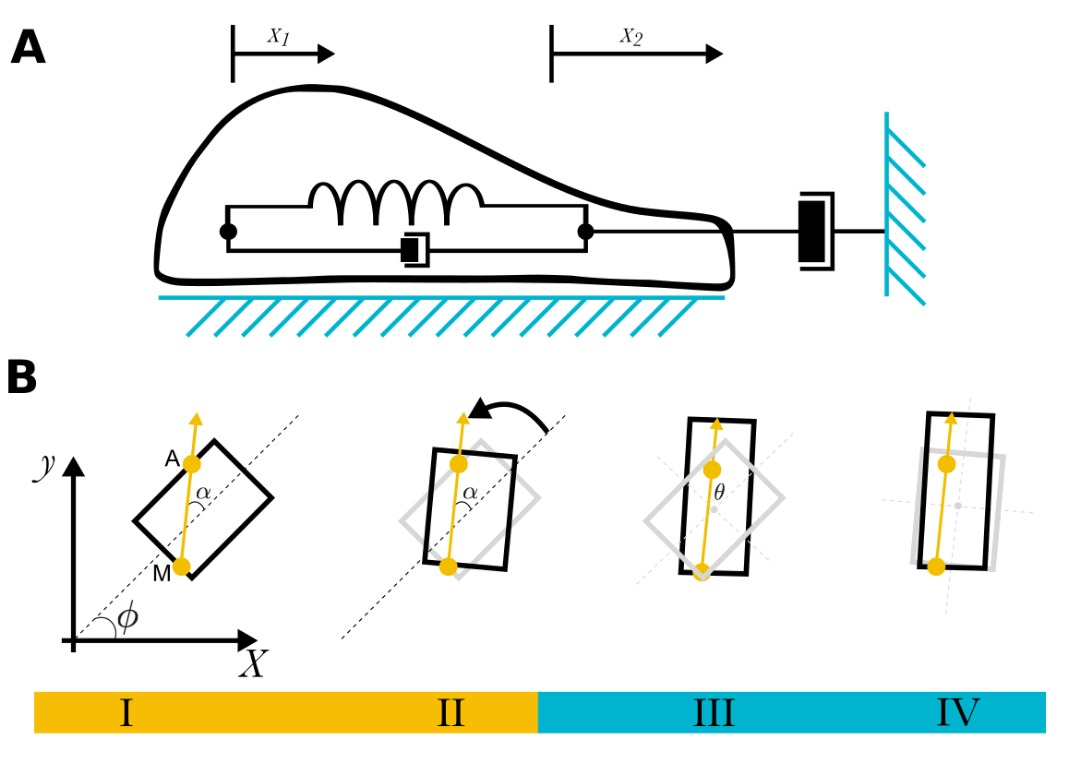
\includegraphics[scale=0.35]{Fig2.jpeg}
\caption{The consecutive steps of cell motility.}
\label{Fig.2}
\end{figure}

\subsection*{The mechanical level}
The myriad of chemical reactions seething at the chimical level should be translated into a physical force to move the cell in a givern direction. But this seemingly trivial step requires further consideration, since the bioligical reality of ameaboid movement is far from simple. To capture some of this apparent biological complexity in our model, the mere act of locomotion is further divided into two steps:


\begin{enumerate}

\item \textit{Deformationl}: To describe cellular deformation we apply sequential geometric transformations including translation, rotation and scaling.\\
When the direction of polarization vector ascertained by chemical level, it is time to move.However, if the length of this ector would be less than a given threshold, howbeit the cells wiggles around, this can not  lead to the movement of the centroid. Morover, if the distance of polarization vector and centroid would be significant, Traction forces provoke rotation of whole cell body around the centroid. Hence, the final direction of cell displacement deviates somehow from the polarization direction dictated from chemical reactions. The amount of this deviation equals to  
\begin{equation}
\Delta \theta=\int_{0}^{t} \omega dt
\end{equation}
in which $\omega$ is anular velocity. As the  movement occures in low Reinolds number regime it is convenient to ignore angular acceleration due to this rotation. Accordingly, one can assume that  total external torque $\tau$ equals to rotational resistance
\begin{equation}
\alpha \omega=\tau
\end{equation}
where $\alpha$ is rotational friction coefficient. Assuming that $F=F_f -F_r$ whre $f_f$ and $f_r$ are  frontal traction force and backward traction force, respectively and $r_{\perp}$ is the distance from centroid from plarization vector, then
\begin{equation}
\Delta \theta=\frac{1}{\alpha}r_{\perp}F t
\end{equation} 
 Here, t is a step time which is a exponential variable with 10 second mean.\\
Now, the amorphous ameoboid cell can adjust itself along the new direction. The length of this step is determined by the interaction of adhesive forces between cell and substrate ( see next subsection). In our model the cell readjustment in a polarized form along a new direction occurs by rotating the previous polarization vector around the meet point of new one ( see \ref{Fig.2}-B-Panel II and supplementary material...). Afterwards, the whole cell rearranges around the new direction such that the area size of the rectangle remains constant (see supplementary material).

\begin{table}[!ht]
\begin{adjustwidth}{0in}{0in} % comment out/remove adjustwidth environment if table fits in text column.
\centering
\caption{{\bf  Biologically meaningful ranges for the model parameters.}}
\begin{tabular}{l   l l l}
\hline\hline
 \textbf{Parameters}&\textbf{Description}  &  \textbf{$Values$} & \textbf{Ref.} \\ \hline
$\gamma_{in}$&Internal Friction Coefficient  &  $10^4~ \mu m pa s$ & $ref$  \\
$\gamma_{out}$&External Friction Coefficient  &  $10 ~\mu m pa s$ & $ref$  \\
$A$& Cell Area  &  $ 100~\mu m^2$ & $ref$  \\
$\eta_{water}$&Water Viscosity &  $10^{-3}~ Pa.s$ & $ref$  \\
$\eta_{cell}$& Cell 's Viscosity &  $10^3-10^5~  Pa.s$ & $ref$  \\
$F_{f}$& Frontal Traction Force  &  $150~ pN $ & $ref$  \\
$F_{r}$& Backward Traction Force  &  $ 120~ pN$ & $ref$  \\
$\omega$& Rotational velocity  &  $4 ~min^{-1}$ & $ref$  \\ 
$\alpha$& Rotational Friction Coefficient  &  $25~ \mu m pN min$ & $ref$  \\
$k$& Cell membrane elasticity &  $10~\mu m Pa$ & $ref$  \\ \hline

\end{tabular}
\label{tab1}
\end{adjustwidth}
\end{table}
\item \textit{Displacement}:
  The entire chain of  intracellur chemical reactions lead us to two distinct  loci, formally we named them the center of actins and the center of myosins. We assume that the center of actins specifies the leading edge of the cell while the center of myosins highlights the rear side of that. these luci represent polarization inside the cell  and the arrow which points the rear edge to the leading one determines the orientation of the cell motility in the next step.\\
%The sequential mechanisms - protrusion, adhesion, and contraction - are acting together to produce cell movement. First, the actin polymerization leads to the extension of the cell’s leading edge. Then, adhesion of the cytoskeleton to the substrate starts to changesuch that the adhesion to the surface at the front gets stronger, than at the cell’s back. Afterwards, the cytoskeleton contracts, pulling the back of the cell forward.\\
Let us model a motile cell  as a viscously damped two degrees of freedom spring-mass system moving forward interacting with substrate, as shown in Fig.(\ref{Fig.2}-A). Since the ahesive forces with substrate is strong enough it is plausible that we assume that the dynamic of the system is over damped and under this condition one can ignore the masses and just follow dyanamics of  the dashpots and the spring . The motion of the system can be describe by the coordinates $x_1(t)$ and $x_2(t)$ which defines the positions of Actin and Myosin centers, \textit{i.e.} head and tail of the cell at any time \textit{t} from the respective equilibrium positions. %The free body diagram of the points are shown in Figure....\\
 The traction forces exerted by the cell provides propulsion force to move forward. This motion is described by the set of coupled diffrential equations
\begin{equation}
-\gamma_{in}(\dot{x_2}-\dot{x_1})-k(x_2-x_1)=-F_r,
\end{equation}
\begin{equation}
\gamma_{in}(\dot{x_2}-\dot{x_1})+k(x_2-x_1)+\gamma_{out}\dot{x_2}=F_f
\end{equation}
where $\gamma_{in}$ and $\gamma_{out}$ are internal and external friction coefficients, respectively and $k$ is the cell membrane elasticity.
\end{enumerate}


\subsection*{Code availability}

\section*{Results}
\subsection{Homogeneous Medium}
\subsection{Inhomogeneous Medium}

\section*{Discussion}
\begin{enumerate}

\item an step forward to have More realistic insight, merely focusing on circumference rather intricate crowded cytoplasm.
\item makes it possible to rebuild the mutation effects.
\item sensitivity of our model to minute assymetry of external concentration gradient
\item All the previous  directional sensing models possess a diffusing communicator agent in cytosol medium of the cell which has not been identified yet, experimentally.
\item Our model assumes that at any instant the cells only grow one pseudopodium, which is not the case in very shallow gradients.
\end{enumerate}



\section*{Supporting information}

\section*{Acknowledgments}

\section*{Author contribution}


\section*{Funding}
This research did not receive any specific grant from funding agencies in the public, commercial, or not-for-profit sectors.

\section*{Additional information}
The authors declare no competing interests. 





\nolinenumbers



% Either type in your references using
 \begin{thebibliography}{}
 \bibitem{Brunet-2016}
Brunet T,and  Arendt D. 2016 From damage response to action potentials: early evolution of neural and contractile modules in stem eukaryotes. Phil. Trans. R. Soc. B 371:2050043
\bibitem{Devreotes-2003}
P. Devreotes and C. Janetopoulos. Eukaryotic chemotaxis: Distinctions between directional sensing and polarization. J. Biol. Chem., 278(23):20445–20448, 2003. 
\bibitem{Meili-2015}
Meili R. , Ellsworth C. , Lee S. , Reddy T. B. , Ma H. , Firtel R. A. Chemoattractant-mediated transient activation and
membrane localization of Akt/PKB is required for
efficient chemotaxis to cAMP in Dictyostelium. (1999) EMBO J. 18:2092–2105
\bibitem{leg1} A. Levchenko, P. Iglesias, Models of Eukaryotic Gradient Sensing:Application to Chemotaxis of Amoebae and Neutrophils, 82, 50-63, 2002.
\bibitem{leg2} C. A. Parent, P. N. Devreotes, A cell's sense of direction, Science, 284, 765-770, 1999.
\bibitem{leg3} B. Kutscher, P. Devreotes, P. A. Iglesias, Local excitation, global inhibition mechanisms for gradient sensing:an interactive applet, Sci STKE, 2004.
\bibitem{leg4} H. Levine, D. A. Kessler, W. J. Rappel, Directional sensing in eukaryotic  chemotaxis: a balanced inactivation model, Proc Natl Acad Sci USA, 103, 9761-9766, 2006.
\bibitem{pol6} M. Postma, P. J. Haastert, A diffusion-translocation model for gradient sensing by chemotactic cells, Biophys J, 81, 1314-1323, 2001.
\bibitem{pol7} A. Gamba, A. de Candia, S. Di. Talia, A. Coniglio, F. Bussolino, G. Serini, Diffusion-limited phase sepration in eukaryotic chemotaxis, Proc Natl Acad Sci USA, 102, 16927-16932, 2005.
\bibitem{pol8}  J. Xu et al, Divergent signals and cytoskeletal assemblies regulate self-organizing polarity in neutrophils, Cell, 114, 201-214, 2003.
\bibitem{cop1} P. J. M. van Haastert, I. K. Gunnink, A. Kortholt, Coupled excitable Ras and F-actin activation mediates spontaneous pseudopod formation and directed cell movement, Mol Biol Cell, 28, 922-934, 2017.
\bibitem{pol1} R. Skupsky, W. Losert, R. J. Nossal, Distinguishing modes of eukaryotic gradient sensing, Biophys J, 89, 2806-2823, 2005.
\bibitem{pol2} X. Xu, M. Meier-Schellersheim, J. Yan, T. Jin, Locality controlled inhibitory mechanisms are involved in eukaryotic GPCR-mediated chemosensing, J. Cell Biol, 178, 141-153, 2007.
\bibitem{pol3} J. E. Ferrell, Self-perpetuating states in signal transduction: positive feedback, double-negative feedback and bistability, Curr Opin Cell Biol, 14, 140-148, 2002.
\bibitem{pol4} A. Narang, Spontaneous polarization in eukaryotic gradient sensing: a mathematical model based on mutual inhibition of frontness and backness pathway, J Theor Biol, 240, 538-553, 2006.
\bibitem{pol5} H. Meinhardt, Orientation of chemotactic cells and growth cones: models and mechanisms, J Cell Sci, 112, 2867-2874, 1999. 
\bibitem{Rappel-2012}
Loomis WF, Fuller D, Gutierrez E, Groisman A, Rappel W-J (2012) Innate Non-Specific Cell Substratum Adhesion. PLoS ONE 7(8): e42033. doi:10.1371/ journal.pone.0042033

 \end{thebibliography}
%
% or
%
% Compile your BiBTeX database using our plos2015.bst
% style file and paste the contents of your .bbl file
% here. See http://journals.plos.org/plosone/s/latex for 
% step-by-step instructions.
% 
%\bibliography{refs}


\end{document}